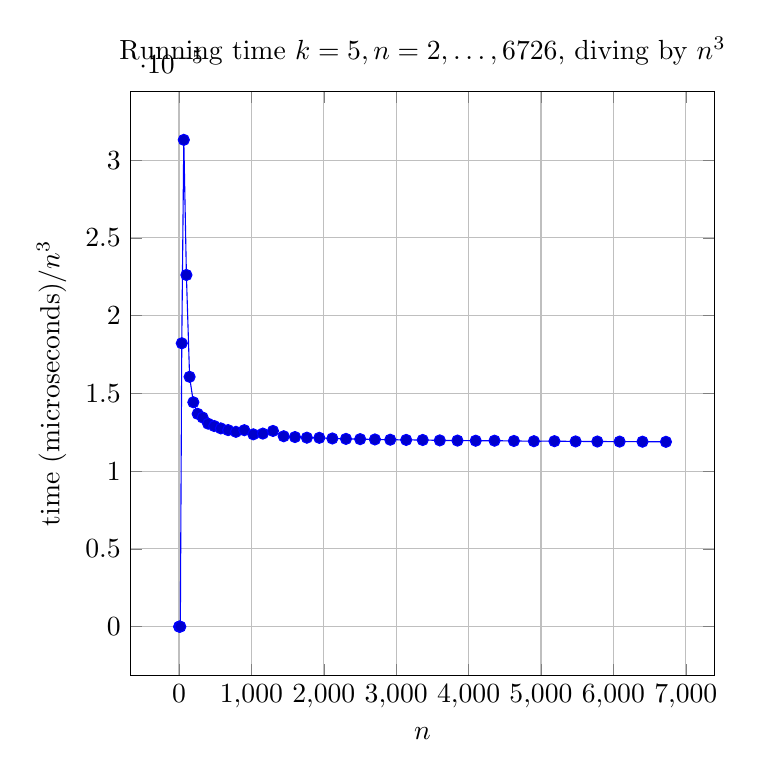
\begin{tikzpicture}
\begin{axis}[
		title={Running time $k=5,n=2,\dots,6726$, diving by $n^3$},
height=9cm,
width=9cm,
grid=major,
xlabel = $n$,
ylabel = time (microseconds)/$n^3$,
]
\addplot coordinates {
	(2,0)
	(6,0)
	(18,0)
	(38,1.82242309374544E-05)
	(66,3.13047833708991E-05)
	(102,2.26157360291291E-05)
	(146,1.60661359272217E-05)
	(198,1.44285421297971E-05)
	(258,1.36838638480003E-05)
	(326,1.34503354733029E-05)
	(402,1.3053221060855E-05)
	(486,1.29016795495295E-05)
	(578,1.27498340864401E-05)
	(678,1.26385397648696E-05)
	(786,1.25270894447943E-05)
	(902,1.26330137388433E-05)
	(1026,1.2367070702209E-05)
	(1158,1.24147019560424E-05)
	(1298,1.25841634982224E-05)
	(1446,1.2243570102851E-05)
	(1602,1.21927454179994E-05)
	(1766,1.2152027041557E-05)
	(1938,1.21417937429069E-05)
	(2118,1.21006985351175E-05)
	(2306,1.20738331437455E-05)
	(2502,1.20580136097767E-05)
	(2706,1.20383485707373E-05)
	(2918,1.20210667777948E-05)
	(3138,1.20081459851104E-05)
	(3366,1.20034459584254E-05)
	(3602,1.19773474781993E-05)
	(3846,1.19642236814143E-05)
	(4098,1.19564913967957E-05)
	(4358,1.19582904652676E-05)
	(4626,1.19410690659842E-05)
	(4902,1.19248646628465E-05)
	(5186,1.19268580687987E-05)
	(5478,1.19119836093996E-05)
	(5778,1.19047328401354E-05)
	(6086,1.1899605218836E-05)
	(6402,1.18935399250374E-05)
	(6726,1.18851040850164E-05)
};
\end{axis}
\end{tikzpicture}
